%!TEX root = ../thesis.tex
\chapter{Introduction}
\label{ch:introduction}

%\epigraph{``As buds give rise by growth to fresh buds, and these, if vigorous, branch out and overtop on all sides many a feebler branch, so by generation I believe it has been with the great Tree of Life, which fills with its dead and broken branches the crust of the earth, and covers the surface with its ever-branching and beautiful ramifications.''}{Charles Darwin, 1872}

\emph{On the Origin of Species} contains a single figure, depicting the ancestry of species as a branching genealogical tree \cite{Darwin:1859uh} (see Figure \ref{fig:darwin_origin}).
Since then, the tree structure has been the dominant framework to understand, visualize, and communicate discoveries about evolution.
Indeed, a primary aim of evolutionary biology has been to expand and fill out what is referred to as the \emph{universal tree of life}, the set of evolutionary relationships among all extant organisms on Earth \cite{Bowler:2003uz}.
Traditionally, this was the realm of phenotype-derived taxonomies [cite].
With the advent of molecular data and numerical approaches for tree-inference, evolutionary biology has become a bona fide quantitative discipline.
Molecular phylogenetics --- tree building --- has become the standard tool for inferring evolutionary relationships.
Yet a tree is only accurate if the Darwinian model of descent with modification via reproduction is the sole process driving evolution.
However, it has long been recognized that there exist alterative evolutionary processes that allow organisms to exchange genetic material through alternative means.
Notable examples including species hybridization, horizontal gene transfer in bacteria, and meiotic recombination in eukaryotes.
Increasing genomic data, powered by new high-throughput sequencing technologies, has shown that these nonvertical processes occur much more frequently than previously believed.
Some have argued that this new data means we need new ways of thinking beyond the tree paradigm [cf. Doolittle].

The aim of this thesis is to present new mathematical and computational tools to study evolution in a variety of contexts.
In the following brief introduction, we survey salient aspects of molecular evolution, the tree paradigm, and challenges thereof.
We then introduce the idea of thinking of evolution as a topological space.

\begin{figure}
\centering
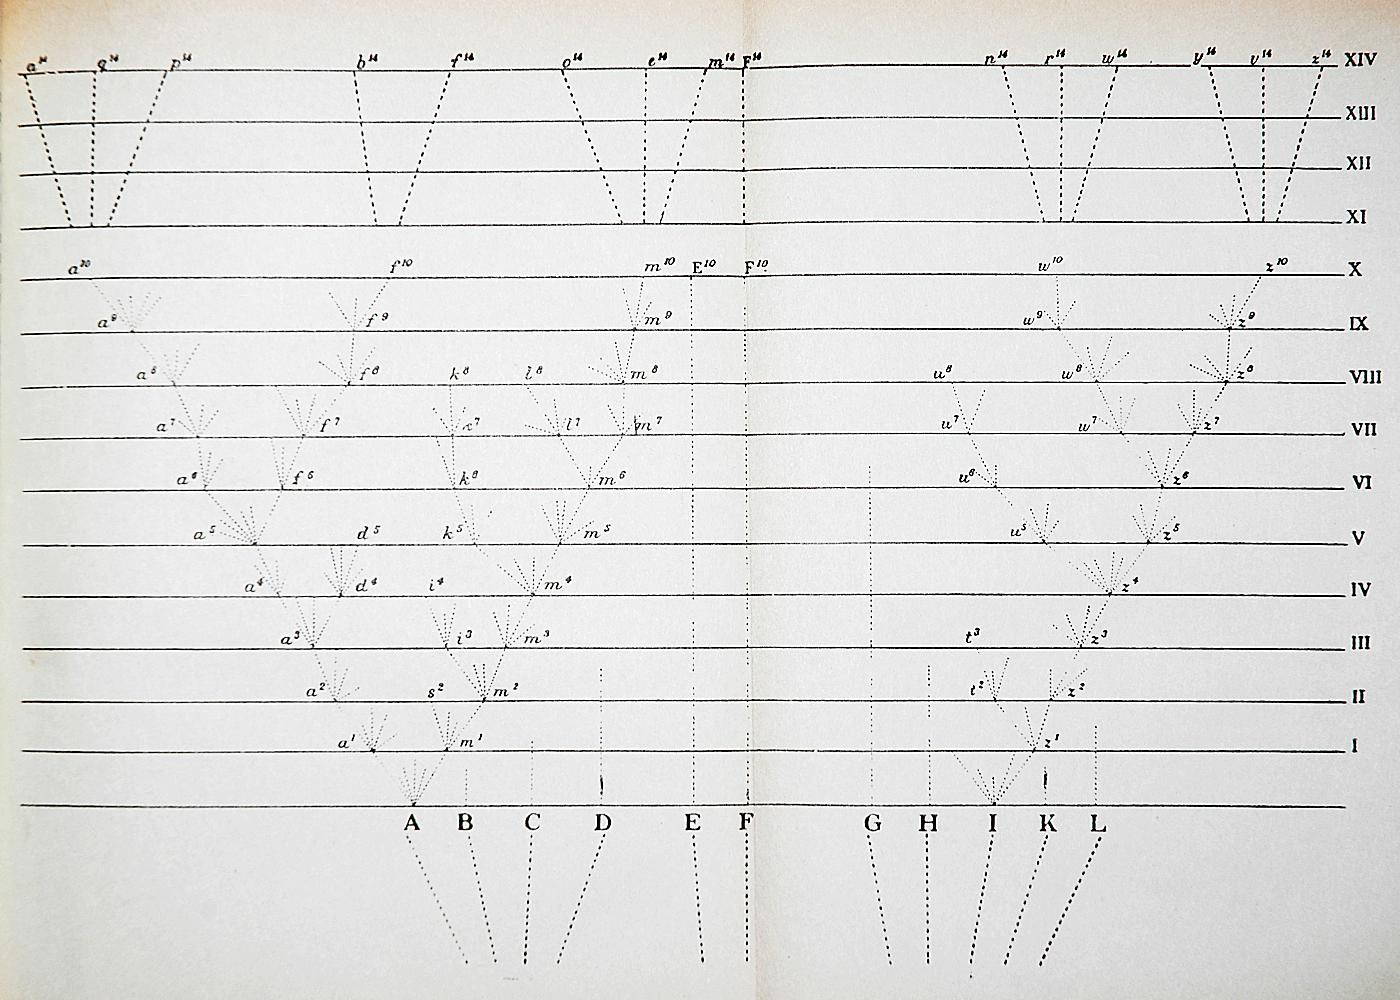
\includegraphics[width=.75\columnwidth]{./fig/introduction/Darwin_divergence.jpg}
\caption[Charles Darwin's Tree]{The only figure in Darwin's Origin of Species.}
\label{fig:darwin_origin}
\end{figure}

\section{Molecular Evolution and the Tree Paradigm}

Molecular evolution: mutation, drift, neutral theory.
The molecular basis of evolution.
Information encoded in DNA, genomes.
Modern evolutionary synthesis: Darwin+Mendel.
Quantitative modeling.
Phylogenetics.
Carl Woese and tree of life
Species, Organism, and Evolution. HGT+Species concepts. Woese+Goldenfeld.
Cosmopolitan genes: move around with environmental pressures [not lineage specific but environment specific.]
Darwin: evolution in terms of organisms not molecules [Pace2009]
Gene tree disconcordance.
How to make a molecular phylogeny? 1. align, 2. evaluate differences; 3. fit a topology

The field was placed on quantitative foundations with the Watson and Crick's discovery of the DNA double-helix in 1953 \cite{Watson:1953wm} and Zuckerkandl and Pauling's recognition that the information encoded in these sequences could be used as a document of evolutionary history in the early 1960's \cite{Zuckerkandl:1962,Zuckerkandl:1965wi}. [NOTE: study microorganisms to probe past evolutionary events; see:Pace2009]
This inaugurated the field of molecular phylogenetics: the comparison of macromolecular sequences to infer genealogies and evolutionary relationships.
With theoretical foundations in place, evolutionary biology progressed in earnest.
Numerical approaches to infer phylogenies were established by Cavalli-Sforza and Edwards in the 1960s.

\kje{(Here insert more of the Doolittle story.)}

molecular phylogenetics — the comparison of macromolecular sequences to infer genealogical and thereby, evolutionary relationships

Carl Woese's later organization of bacteria, eukarya, and archaea into the three domains of life was based on only 1,500 nucleotides in the 16S subnit ribosomal RNA, less than 0.00005\% of the human genome \cite{Woese:1977vd}
More recent work developed automated approach yadda yadda\cite{Ciccarelli:2006gw}, but even then that is only 0.01\% of a typical human genome, as articulated in Dagan/Martin tree of 1\% \cite{Dagan:2006up}.

These nonvertical modes of evolution are more than just a theoretical concern:
In HIV, frequent recombination confounds our understanding of the early and present epidemic’s history. [cite]
In influenza, gene reassortments lead to antigenic novelty and the emergenence of epidemics. [cite]
Horizontal gene transfer has been largely responsible for the spread of antibiotic resistance in pathogens of concern, including E. coli and S. aureus. [cite]

One wonders if the information deduced from small genomic sections can be extrapolated to other regions, as different gene sequences can yield vastly different tree topologies.
Incompatibilities in the tree model now appear as the rule, not the exception, demonstrating the need for new representations of evolutionary relationships \autocite{Doolittle:1999,Doolittle:2006}.
These and other similar situations, further described below, call for new methods of characterizing evolutionary relationships.

Many have argued that, in light of genomic evidence of HGT, the very notion of a universal tree of life must be discarded. \kje{[cite Doolittle, Koonin]}.

sequences of orthologous genes! [plug that stuff into Ayasdi!]

\begin{figure}
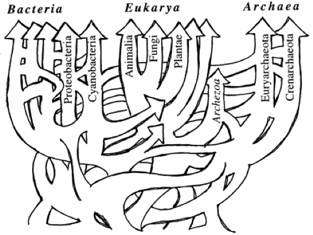
\includegraphics[width=\columnwidth]{./fig/introduction/doolittle_tree.png}
\caption[Ford Doolittle's Tree]{W Ford Doolittle's representation of the universal tree of life with nonvertical evolution. (From \emph{Science}, vol. 284, issue 5423, page 2127. Reprinted with permission from AAAS.)}
\label{fig:doolittle_tree}
\end{figure}

In this thesis, we propose the use of new computational techniques, borrowed from the field of algebraiac topology, to capture and represent complex patterns of genetic exchange that may be obscured using current phylogenetic approaches and tree-centered thinking.

\section{Evolution as a Topological Space}

In this thesis, we propose the use of new computational techniques, borrowed from the field of algebraic topology, to capture and represent complex patterns of genetic exchange.


While this may appear obscure at first glance, let us unpack the idea.
Topology is concerned with invariant properties of spaces.
The paradigmatic example is the circle.
Algebraic topology assigns algebraic quantities to these properties and lets us speak and compare spaces quantitatively.

Consider again Darwin's branching phylogeny in Figure \ref{fig:darwin_origin}.
Consider Doolittle's net of life.
Much more complicated topological space.
If we envision these relationships as a topological space, we could use a similar characterization.
The tree is trivially compactable.
An evolutionary scenario which includes nonvertical processes

there are complications that must be addressed at the outset.
First, deep evolutionary history consists of extinct organisms.
[By the way, how old is life? Mention that.]
Second, we do not have complete sampling.
Third, not all organisms have compatible gene sets to make comparisons.
This is of course why Woese focused on conserved ribosomal RNA, some of the oldest genomic information.

\begin{figure}
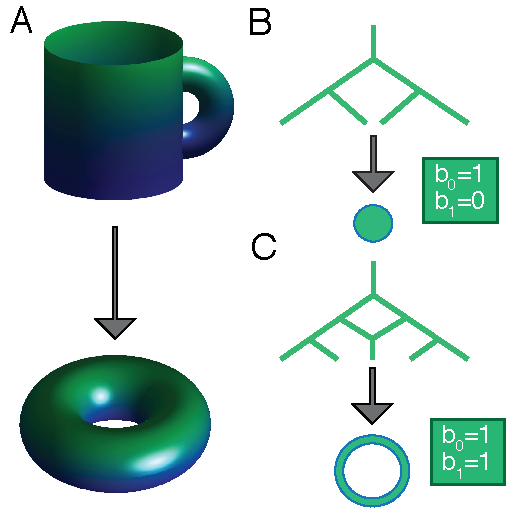
\includegraphics[width=\columnwidth]{./fig/introduction/topology_example.pdf}
\caption[The Paradigmatic Topology Example]{The coffee cup is not trivially contractible. The tree is contractible. The network is not contractible. Betti numbers quantitatively capture these notuons of shape.}
\label{fig:topology_example}
\end{figure}

In this thesis, we use new computational techniques, borrowed from the field of algebraic topology, to capture and represent complex patterns of gene exchange that are obscurbed in current phylogenetic methods.
By doing so, we provide a fuller understanding of evolutionary relationships than allowed by current phylogenetic methods.
Genomic exchange can be characterized by the parental sequences involved in the exchange, by the amount and identity of material exchanged (i.e., the genes or loci involved), and the frequency with which similar exchanges occur.
Techniques such as phylogenetic networks and ancestral recombination graphs have been developed to describe reticulate evolution, but they have had only limited success due to difficulties of biological interpretation and computational infeasibility in all but the smallest datasets.

Should I give a simple description of constructing additive trees

Linkage-based techniques have succeeded in measuring rates of recombination in medium-sized datasets (< 200 sequences), but they cannot reveal the scale of these exchanges (i.e., the genetic distance between parental sequences), and they have limited resolution in pinpointing where along a genome such exchanges have occurred.
A new mathematical foundation is needed to break free of these limitations.

Genome evolution is an extremely rich subject [cite Genome Architecture book].

This thesis contains results of applying methods from topological data analysis to various problems in genomics and evolution.
It primarily details the use of persistent homology as a tool to measure the prevalence and scale of nonvertical evolutionary events, such as reassortments and recombinations.
In so doing, various techniques are developed to extract statistical information from the topological complexes that are constructed.

\section{Thesis Organization}

The remainder of this thesis is organized as follows.

In Chapter \ref{ch:background} we present background information on the wide range of topics discussed in this thesis.
This discussion is chiefly structured into two pieces: (1) background on phylogenetics and population genetics, and (2) background on algebraic topology and the methods of topological data analysis.

In Part \ref{part:theory}, we develop two complementary approaches for analyzing genomic data using topological data analysis.
In Chapter \ref{ch:parametric_inference}, we develop methods for performing statistical inference using summary statistics contained in the persistence diagram.
This is the first such use of persistence diagrams as a tool for performing parametric inference.
In Chapter \ref{ch:complex_construction}, we propose alternative methods of constructing topological complexes that generalize the traditional Vietoris-Rips and \Cech complexes but are suited to the particular demands of phylogenetic applications.
We draw on previous work in phylogenetic networks and use homology theory to provide quantitative assessment of reticulation.

In Part \ref{part:application_microorganism} we apply our approach various microorganism datasets.
In Chapter \ref{ch:phage} we study bacteriophages.
In Chapter \ref{ch:influenza} we study influenza.
In Chapter \ref{ch:pathogens} we study pathogenic bacteria and use topological techniques to represent the spread of antibiotic resistance.
In Chapter \ref{ch:prokaryotes} we study prokaryotes.

In Part \ref{part:applications_human}, we apply our approaches to a several problems in human population genetics and biology.
In Chapter \ref{ch:human_recombination_rate} we measure the human recombination rate.
In Chapter \ref{ch:human_population_structre} we reconstruct models of human demographic movements.
In Chapter \ref{ch:human_chromatin_folding} we analyze Hi-C data to understand patterns of chromatin folding in the nucleus.

Finally, in Chapter \ref{ch:conclusions} we summarize our results and present possible avenues for future directions.